\documentclass[11pt,a4paper]{article}

\usepackage[T1]{fontenc}
\usepackage{amsmath,amssymb,amsthm}
\usepackage[margin=3cm]{geometry}
\usepackage{mathtools}
\usepackage{graphicx}
\usepackage{booktabs}
\usepackage[hidelinks]{hyperref}

\graphicspath{{../}}

%% --------------------------------------------------------------------------
%%  Bourbaki-style numbering (matching the repo convention).
%% --------------------------------------------------------------------------
\newtheoremstyle{bourbaki}{\topsep}{\topsep}{\itshape}{}{\scshape}{.}{ }{}
\newtheoremstyle{bourbakidef}{\topsep}{\topsep}{\upshape}{}{\scshape}{.}{ }{}
\theoremstyle{bourbaki}
\newtheorem{thm}{Theorem}[section]
\newtheorem{prop}[thm]{Proposition}
\newtheorem{lem}[thm]{Lemma}
\newtheorem{cor}[thm]{Corollary}
\theoremstyle{bourbakidef}
\newtheorem{defn}[thm]{Definition}
\newtheorem{rem}[thm]{Remark}
\newtheorem{conj}[thm]{Conjecture}
\renewcommand{\qedsymbol}{$\blacksquare$}

\newcommand{\Z}{\mathbb{Z}}
\newcommand{\N}{\mathbb{N}}
\newcommand{\Q}{\mathbb{Q}}
\newcommand{\R}{\mathbb{R}}
\newcommand{\HH}{\mathbb{H}}
\newcommand{\Emink}{\mathbb{E}^{1,2}}
\newcommand{\slt}{\mathfrak{sl}_2(\R)}
\newcommand{\Teich}{\mathcal{T}}
\DeclareMathOperator{\Ad}{Ad}
\DeclareMathOperator{\tr}{tr}
\DeclareMathOperator{\SO}{SO}
\DeclareMathOperator{\SL}{SL}
\DeclareMathOperator{\PSL}{PSL}
\DeclareMathOperator{\Isom}{Isom}
\DeclareMathOperator{\Fix}{Fix}
\DeclareMathOperator{\Reg}{Reg}
\newcommand{\Span}{\operatorname{span}}

\title{The flat Lorentzian spacetime of the Syracuse cycle problem:\\
       a closed geodesic with extreme BTZ}
\author{L\'eo Brunswic}
\date{20 June 2026}

\begin{document}
\maketitle

\begin{abstract}
We give a geometric reformulation of the cycle problem for the Syracuse (Collatz) map.
The two affine maps $a:z\mapsto\tfrac{3z+1}{2}$ and $b:z\mapsto\tfrac{z}{2}$ generate a
free group $F_2=\pi_1(\Sigma_{1,1})$, the fundamental group of the once--punctured torus;
the Collatz cocycle $S$ together with the integer $D=2^E-3^o$ packages the cycle equation
as the divisibility $D\mid S$. Realising $F_2$ inside the affine isometry group of
Minkowski $3$--space $\Emink=\slt$ identifies the data with a globally hyperbolic,
Cauchy--compact, \emph{future--complete} flat Lorentzian spacetime carrying exactly one
\emph{extreme BTZ} singular line at the puncture --- an object of the classification of
\cite{Brunswic2021}, a point of the tangent bundle $T\Teich(\Sigma_{1,1})$. In this model
$D$ is a Minkowski interval, the critical band $2^E\approx 3^o$ is the light cone, and the
Collatz cocycle $S$ is the lightlike translation (the BTZ datum). Each primitive conjugacy
class is a closed \emph{spacelike} geodesic; we show that the Syracuse cycles are exactly
those geodesics whose ideal endpoint on the null boundary is an \emph{integer}
(equivalently $x_0^\ast=S/D\in\Z$). All quantitative claims are machine--certified.
\end{abstract}

\section{Introduction}

The Syracuse (Collatz, $3x+1$) map sends an odd integer $a$ to the odd part of
$3a+1$. Its \emph{accelerated} form is generated by the two affine maps of the line
\begin{equation}\label{eq:gens}
  a:\ z\longmapsto \frac{3z+1}{2},\qquad b:\ z\longmapsto \frac{z}{2},
\end{equation}
both elements of the affine group $\mathrm{Aff}(\R)=\R\rtimes\R^\times$. A trajectory is a
word in $\{a,b\}$, and a \emph{cycle} is a closed word fixing an integer. The two maps
generate a free group of rank two,
\[
  F_2=\langle a,b\rangle\ \cong\ \pi_1(\Sigma_{1,1}),
\]
the fundamental group of the once--punctured torus. This coincidence is the starting point:
closed words become free homotopy classes of closed curves, and the cycle problem becomes a
\emph{closed geodesic problem} --- once a geometric structure realising $a,b$ is fixed.

Two affine maps with different linear parts ($\times\tfrac32$ versus $\times\tfrac12$) are
not isometries of one hyperbolic metric, and one checks (\S\ref{sec:model}) that the
hyperbolic uniformisation is obstructed: the generators are \emph{sub-Markoff}. The correct
ambient geometry is \emph{Lorentzian}. We place $F_2$ inside the affine isometry group of
Minkowski $3$--space and obtain the following picture, whose pieces are made precise below
and certified by the scripts of the appendix.

\begin{thm}[Informal]\label{thm:informal}
The Syracuse data determines a globally hyperbolic, Cauchy--maximal, Cauchy--compact,
future--complete flat Lorentzian $3$--manifold $M$, homeomorphic to $\Sigma_{1,1}\times\R$,
with exactly one extreme BTZ singular line at the puncture --- a point of
$T\Teich(\Sigma_{1,1})$ in the classification of \cite{Brunswic2021}. In $M$:
\begin{enumerate}
\item $D=2^E-3^o$ is the Minkowski interval, and the critical band $2^E\approx 3^o$ is the
      light cone;
\item the Collatz cocycle $S$ is the lightlike (BTZ) translation cocycle;
\item every primitive conjugacy class is a closed spacelike geodesic, and a class is a
      \emph{Syracuse cycle} if and only if its geodesic has an integer ideal endpoint
      $x_0^\ast=S/D$ on the null boundary.
\end{enumerate}
\end{thm}

\section{The Syracuse cocycle}\label{sec:cocycle}

We recall the cocycle calculus underlying the cycle equation; see
\cite{BohmSontacchi,Brunswic2021} and the project's structural notes.

Encode a trajectory by its \emph{gap word} $w=(d_0,\dots,d_{o-1})$ of positive integers:
$o$ is the number of odd steps, $d_k$ the number of halvings at the $k$--th step, and
$E=\sum_k d_k$ the total number of halvings. With partial sums
$e_k=\sum_{i<k}d_i$ set
\begin{equation}\label{eq:SD}
  S(w)=\sum_{k=0}^{o-1} 2^{e_k}\,3^{\,o-1-k},
  \qquad
  D(w)=2^{E}-3^{o}.
\end{equation}
Starting from an odd $a_0$ and ending at $a_o$, the closed form of the dynamics is the
linear Diophantine identity $2^{E}a_o-3^{o}a_0=S(w)$. The word map is the affine map
\begin{equation}\label{eq:Fgamma}
  F_w(z)=\frac{3^{o}}{2^{E}}\,z+\frac{S(w)}{2^{E}},
  \qquad\text{with unique fixed point}\quad
  x_0^\ast=\frac{S(w)}{D(w)}.
\end{equation}
A cyclic word is a cycle precisely when this fixed point is the (integer) starting value,
i.e.
\begin{equation}\label{eq:cyclecond}
  \boxed{\ \gamma\text{ is a Syracuse cycle}\iff D(\gamma)\mid S(\gamma)\iff x_0^\ast=S/D\in\Z.\ }
\end{equation}
The functional $S$ is a $1$--cocycle: over $R=\Z[X,Y]$ the word map is the transfer--matrix
homomorphism
\begin{equation}\label{eq:transfer}
  M(w)=\begin{pmatrix} Y^{o} & 0\\ S(w) & X^{E}\end{pmatrix},
  \qquad (X,Y)\mapsto(2,3),
\end{equation}
with $\tr M=X^E+Y^o$, $\det M=X^EY^o$ and eigenvalue gap $X^E-Y^o=D$. On a cycle
$\gcd_j S^{(j)}=|D|$, which is odd. We retain three invariants of a cyclic class $\gamma$:
the pair $(E,o)$, the cocycle value $S$, and the interval $D=2^E-3^o$.

\section{The flat Lorentzian model}\label{sec:model}

Let $\Emink=\slt$ be Minkowski $3$--space, with the $\Ad$--invariant Lorentzian form
\begin{equation}\label{eq:form}
  q(X)=-\det X=\tfrac12\tr(X^2),\qquad \langle X,Y\rangle=\tfrac12\tr(XY),
\end{equation}
of signature $(1,2)$. In the basis
$H=\left(\begin{smallmatrix}1&0\\0&-1\end{smallmatrix}\right)$,
$E=\left(\begin{smallmatrix}0&1\\0&0\end{smallmatrix}\right)$,
$F=\left(\begin{smallmatrix}0&0\\1&0\end{smallmatrix}\right)$ the vector $H$ is spacelike,
$E$ and $F$ are null, and $E-F$ is timelike. The orientation-- and time--orientation--
preserving isometry group is
\[
  \Isom_0(\Emink)=\SO_0(1,2)\ltimes\R^{1,2}=\PSL_2(\R)\ltimes\slt,\qquad
  X\mapsto \Ad(g)X+v,
\]
with $\Ad:\SL_2(\R)\to\SO_0(1,2)$ the adjoint cover. The Syracuse generators
\eqref{eq:gens} lift to $A=\left(\begin{smallmatrix}3&1\\0&2\end{smallmatrix}\right)$,
$B=\left(\begin{smallmatrix}1&0\\0&2\end{smallmatrix}\right)$; after normalisation in
$\SL_2(\R)$ their trace coordinates are
$(\tr A,\tr B,\tr AB)=(\tfrac{5}{\sqrt6},\tfrac{3}{\sqrt2},\tfrac{7}{2\sqrt3})$, whence by
Fricke $\tr[A,B]=+2$. Thus $\langle A,B\rangle$ is \emph{reducible} (the generators share a
boundary fixed point), and all three traces are $<3$: the generators are \emph{sub-Markoff},
so no faithful Fuchsian uniformisation of the cusped once--punctured torus has these traces.
This is the obstruction that rules out the hyperbolic target and selects the Lorentzian one,
which carries no length floor.

The boost spectrum of a cycle is transparent in null coordinates.

\begin{prop}[spectral picture; certified in \texttt{lorentzian.py}]\label{prop:spectral}
Let $\gamma$ be a cyclic class with invariants $(E,o)$ and let $G$ be its (normalised)
holonomy element. Then $\Ad(G)$ has eigenvalues
\[
  \Big\{\ \tfrac{2^E}{3^o},\ 1,\ \tfrac{3^o}{2^E}\ \Big\},
\]
its neutral axis $x^0=G-\tfrac12(\tr G)\,\mathbf 1$ is spacelike ($q(x^0)>0$), and the boost
rapidity equals the hyperbolic length $\ell=\bigl|\log(2^E/3^o)\bigr|$. In the null
coordinates $(u,v)=(2^E,3^o)$ one has $u+v=\tr$, $uv=\det$, and
\[
  D=2^E-3^o=u-v\ \text{is the Lorentzian interval},
\]
so that the critical band $2^E\approx 3^o$ is exactly the light cone $u=v$.
\end{prop}

Figure~\ref{fig:H} shows the companion Riemannian picture
($\mathrm{Aff}_+(\R)\cong\HH$): each cycle is a vertical geodesic ending at $x_0^\ast=S/D$,
of length $\ell$ --- the same boost rapidity.

\begin{figure}[ht]
  \centering
  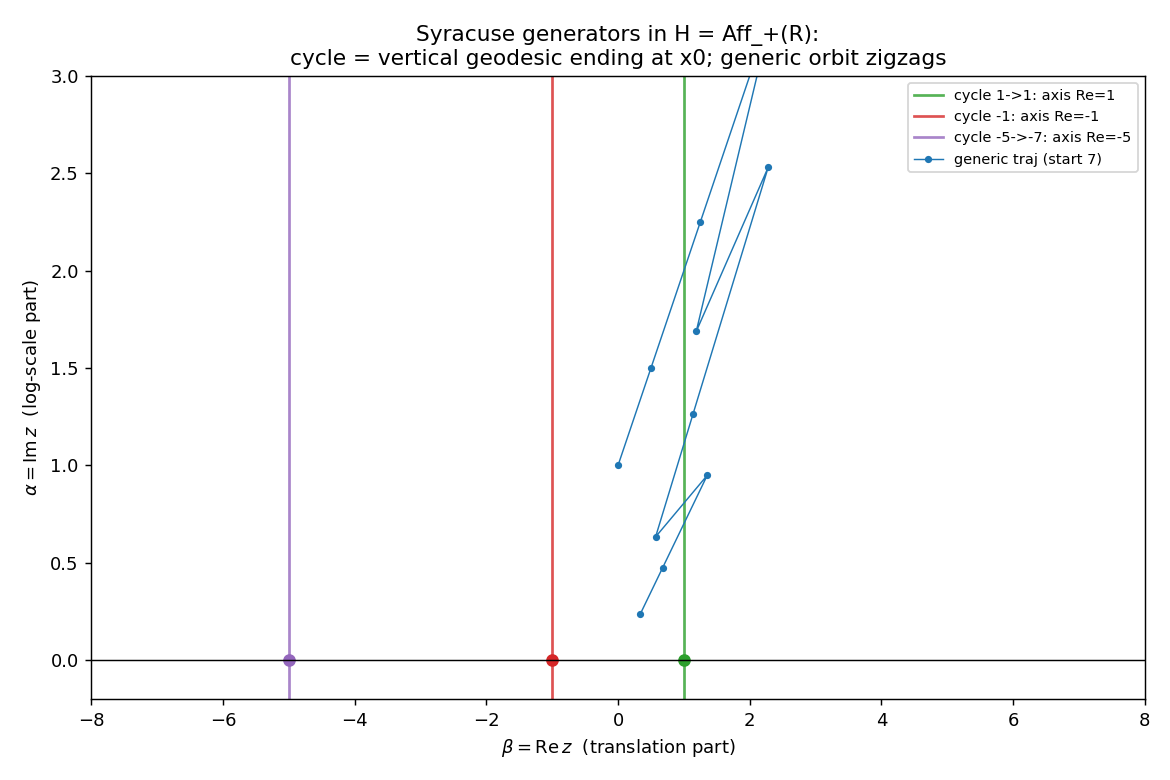
\includegraphics[width=0.74\textwidth]{hyperbolic_model.png}
  \caption{The companion half--plane model $\mathrm{Aff}_+(\R)\cong\HH$. Each Syracuse cycle
  is the vertical geodesic $\mathrm{Re}=x_0^\ast$ ending at its value $x_0^\ast=S/D$, of
  length $\ell=|\log(2^E/3^o)|$; a generic (non--periodic) orbit zigzags.}
  \label{fig:H}
\end{figure}

\section{The representation and the spacetime}\label{sec:rep}

The holonomy is $\rho:F_2\to\PSL_2(\R)\ltimes\slt$, $\rho(\gamma)=(L(\gamma),\tau(\gamma))$,
with linear part $L$ and translation cocycle $\tau$
(\,$\tau(\gamma_1\gamma_2)=\tau(\gamma_1)+\Ad(L(\gamma_1))\tau(\gamma_2)$\,).

\begin{prop}[the translation cocycle; certified in \texttt{spacetime.py}]\label{prop:tau}
Reading off the intercept of \eqref{eq:Fgamma}, the translation cocycle is the Collatz
cocycle itself, valued in the null line $\R\cdot E$:
\[
  \tau(\gamma)=\frac{S(\gamma)}{2^{E(\gamma)}}\,E,
  \qquad \tau(a)=\tfrac12E,\quad \tau(b)=0,\qquad q(\tau)\equiv 0.
\]
\end{prop}

The linear part admits two readings. The \emph{canonical} one is the multiplicative $2$--$3$
skeleton $L_0$ ($\Ad L_0$ a boost fixing $H$: $a:E\mapsto\tfrac32E$, $b:E\mapsto\tfrac12E$);
it is abelian/reducible --- a noded boundary point of $\Teich(\Sigma_{1,1})$. The
\emph{smooth} one is any genuine Fuchsian uniformisation $L\in\Teich(\Sigma_{1,1})$ of the
cusped once--punctured torus. In either case the puncture $[a,b]$ is parabolic
($[A,B]=\left(\begin{smallmatrix}1&1/4\\0&1\end{smallmatrix}\right)$, $\Ad[A,B]$ unipotent
fixing the null line $\R E$) --- the \emph{extreme BTZ} singular line, the Lorentzian cusp.

Over a Fuchsian base, the work of Mess and Bonsante \cite{Mess2007,Bonsante2005} produces the
maximal globally hyperbolic regular domain $\Omega\subset\Emink$ with lightlike support
planes, and $M=\rho(F_2)\backslash\Omega$ is a globally hyperbolic, Cauchy--maximal,
Cauchy--compact flat spacetime; the extreme--BTZ extension of \cite{Brunswic2021} adjoins the
singular line at the cusp.

\begin{prop}[causal type]\label{prop:future}
$M$ carries a regular cosmological time $T:M\to(0,+\infty)$; it is future--complete and
past--incomplete, the initial singularity ($T\to0$) being the $\R$--tree dual to the measured
lamination encoded by $\tau$. The extreme--BTZ line is a white hole on the initial--
singularity side; its time orientation is fixed by the (future--pointing) sign of the
Syracuse $+1$, namely $\tau(a)=+\tfrac12E$.
\end{prop}

\section{Identification in the classification of \texorpdfstring{\cite{Brunswic2021}}{Brunswic}}
\label{sec:brunswic}

The relevant moduli space is parametrised by a tangent bundle of Teichm\"uller space.

\begin{thm}[\cite{Brunswic2021}, Theorem 1]\label{thm:brunswic}
Let $\Sigma^\ast$ be a surface of genus $g$ with $s$ marked points and $2-2g-s<0$. The
deformation space of globally hyperbolic, Cauchy--maximal flat spacetimes homeomorphic to
$\Sigma\times\R$ with exactly $s$ extreme--BTZ singular lines is identified with the tangent
bundle $T\Teich(\Sigma^\ast)$. The base is the Fuchsian linear part $L$; the fibre is the
translation cocycle $\tau\in H^1(\pi_1,\R^{1,2}_{\Ad L})$. Extreme BTZ holonomy is parabolic,
the Lorentzian analogue of a cusp.
\end{thm}

For us $\Sigma^\ast=\Sigma_{1,1}$ is the once--punctured torus: $g=1$, $s=1$, so
$2-2g-s=-1<0$ and Theorem~\ref{thm:brunswic} applies, with $\dim_\R T\Teich=4$. The
dictionary is summarised in Table~\ref{tab:dict}. The single marked point is the puncture,
whose parabolic holonomy is the extreme BTZ; the base point is the Syracuse linear part and
the fibre is the cocycle $S$ of Proposition~\ref{prop:tau}.

\begin{table}[ht]
  \centering
  \begin{tabular}{@{}ll@{}}
    \toprule
    \textbf{\cite{Brunswic2021} object} & \textbf{Syracuse object}\\
    \midrule
    Cauchy surface $\Sigma^\ast$            & once--punctured torus ($g{=}1,s{=}1$, $2{-}2g{-}s{=}{-}1$)\\
    isometry group $\PSL_2\ltimes\R^3$      & affine isometries of $\Emink=\slt$\\
    extreme BTZ (parabolic)                 & the puncture $[a,b]$, $\Ad$--unipotent, null axis $\R E$\\
    base point $\in\Teich(\Sigma^\ast)$     & the linear holonomy (the $2$--$3$ skeleton)\\
    translation cocycle $\tau$              & the Collatz cocycle $S$ (lightlike, $\tau=\tfrac{S}{2^E}E$)\\
    Minkowski interval                      & $D=2^E-3^o$; criticality $=$ light cone\\
    \bottomrule
  \end{tabular}
  \caption{The identification of the Syracuse data with a point of $T\Teich(\Sigma_{1,1})$.}
  \label{tab:dict}
\end{table}

\section{Syracuse cycles as closed geodesics}\label{sec:main}

Free homotopy classes of closed curves on $\Sigma_{1,1}$ are conjugacy classes of $F_2$,
hence cyclic gap words. A class with hyperbolic linear part is a closed \emph{spacelike}
geodesic of $\Reg(M)$, with axis the neutral direction $x^0(\gamma)$ of
Proposition~\ref{prop:spectral} and length $\ell=|\log(2^E/3^o)|$; the parabolic class
$[a,b]$ is the BTZ line. The cycle condition is the integrality of one ideal endpoint.

\begin{prop}[fixed locus; certified in \texttt{spacetime.py}]\label{prop:fix}
At the reducible base the holonomy $(\Ad L_0(\gamma),\tau(\gamma))$ fixes a spacelike line
pointwise,
\[
  \Fix=\bigl\{\,tH+x_0^\ast\,E:\ t\in\R\,\bigr\},\qquad x_0^\ast=\frac{S}{D},
\]
because $\tau$ is null, so the Margulis invariant $\langle\tau,x^0\rangle$ vanishes. The
null--position of this line --- equivalently the geodesic's ideal endpoint on the null
boundary $\partial_\infty=\R\cup\{\infty\}$, on which the BTZ cusp sits at $\infty$ --- is
$x_0^\ast=S/D$.
\end{prop}

\begin{thm}[Property $P$; certified in \texttt{spacetime.py}]\label{thm:P}
The map $\gamma\mapsto(\text{axis of }\rho(\gamma))$ sends primitive cyclic classes to
closed spacelike geodesics of $M$. A class $\gamma$ is a \emph{Syracuse cycle} if and only if
\begin{align*}
  & D(\gamma)\mid S(\gamma)\iff x_0^\ast=\tfrac{S}{D}\in\Z\\
  &\qquad\iff \text{the geodesic has an integer ideal endpoint on the null boundary,}
\end{align*}
a marked point of the lattice $\Z\subset\partial_\infty$ in the parabolic (BTZ--cusp) orbit.
\end{thm}

\begin{proof}[Sketch]
By \eqref{eq:cyclecond} a cyclic class is a cycle iff $x_0^\ast=S/D\in\Z$. By
Proposition~\ref{prop:fix} the number $x_0^\ast$ is exactly the null--position of the fixed
spacelike line, i.e.\ the geodesic's ideal endpoint. Integrality of that endpoint is thus the
cycle condition. The numerical content is certified in \texttt{spacetime.py}.
\end{proof}

The content of Theorem~\ref{thm:P} is illustrated by the five representative classes of
Table~\ref{tab:cycles}: the three Syracuse cycles have integer endpoints $1,-1,-5$; the two
non--cycles have endpoints $\tfrac15,\tfrac57\notin\Z$.

\begin{table}[ht]
  \centering
  \begin{tabular}{@{}lllrrrl@{}}
    \toprule
    class & gap word & $(o,E)$ & $S$ & $D$ & $x_0^\ast=S/D$ & cycle?\\
    \midrule
    $ab$    & $(2)$   & $(1,2)$ & $1$ & $1$  & $1$            & yes\\
    $a$     & $(1)$   & $(1,1)$ & $1$ & $-1$ & $-1$           & yes\\
    $aab$   & $(1,2)$ & $(2,3)$ & $5$ & $-1$ & $-5$           & yes\\
    $abb$   & $(3)$   & $(1,3)$ & $1$ & $5$  & $\tfrac15$     & no\\
    ---     & $(1,3)$ & $(2,4)$ & $5$ & $7$  & $\tfrac57$     & no\\
    \bottomrule
  \end{tabular}
  \caption{Property $P$ on five classes: integer ideal endpoint $\iff$ Syracuse cycle.}
  \label{tab:cycles}
\end{table}

In words: \emph{every conjugacy class is a closed spacelike geodesic, and the Collatz cycle
problem asks which of these geodesics close up over the integer points of the null boundary
attached to the BTZ cusp.} Absence of nontrivial positive cycles is the statement that no
closed spacelike geodesic but the trivial one has a positive integer ideal endpoint.

\section{Status and open questions}\label{sec:status}

The above is exact and certified \emph{at the reducible base}, where however the action is
non--free: the null cocycle makes every Margulis invariant vanish
(Proposition~\ref{prop:fix}), so this base is the noded boundary point of $T\Teich$, not a
smooth spacetime. A smooth Brunswic spacetime requires an interior Fuchsian base $L$ carrying
the same cocycle $\tau=S$; under such a lift the two ideal endpoints become finite and the
Margulis length turns on. Figure~\ref{fig:def} shows the naive (trace--non--increasing)
deformation off the reducible locus: $\tr[A,B]$ bottoms at $+2$ and never reaches the cusped
Fuchsian value $-2$, and the critically short cycles tip to elliptic --- a usable deformation
must lengthen geodesics.

\begin{figure}[ht]
  \centering
  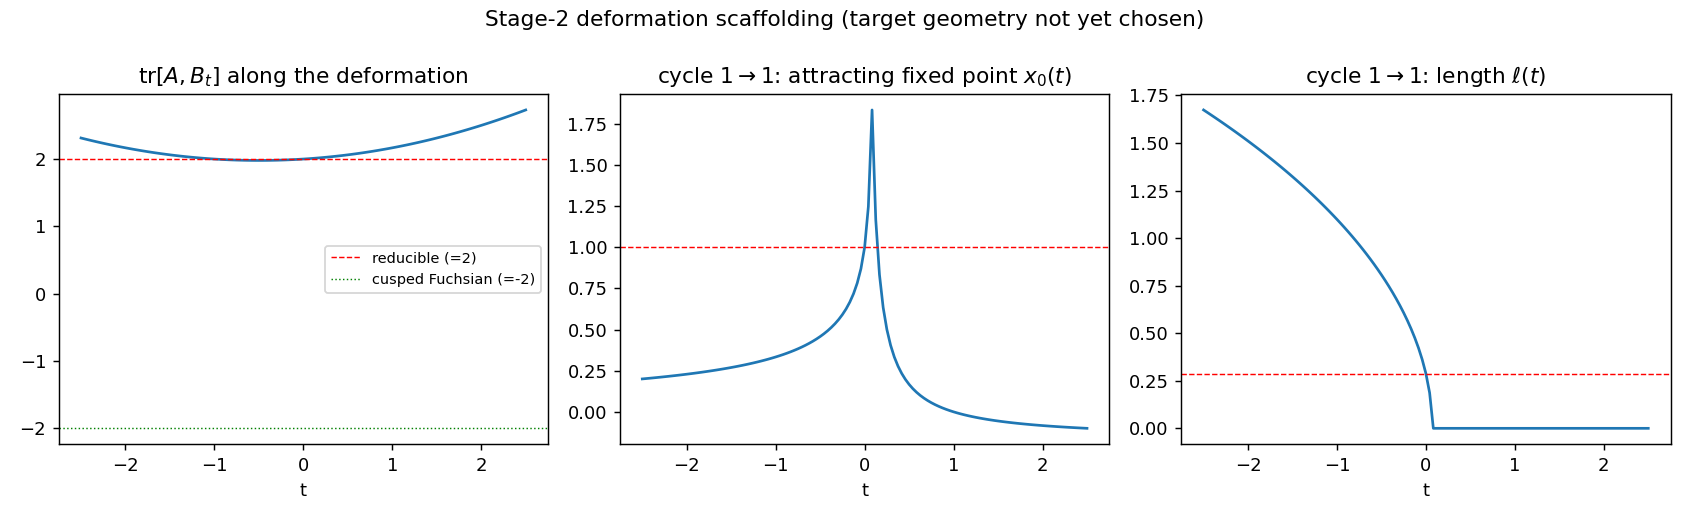
\includegraphics[width=0.96\textwidth]{markoff_deformation.png}
  \caption{Naive deformation off the reducible locus: $\tr[A,B]$ bottoms at $+2$ (never
  reaching the cusped Fuchsian $-2$); the trivial cycle's length collapses (elliptic) as the
  axes separate. The smooth lift must increase the generator traces.}
  \label{fig:def}
\end{figure}

\begin{conj}\label{conj:lift}
There is a Fuchsian base $L\in\Teich(\Sigma_{1,1})$ carrying $\tau=S$ for which the integer
ideal--endpoint condition of Theorem~\ref{thm:P} survives as an intrinsic geometric
statement --- a closed--geodesic return condition, or a BTZ--extension / Cauchy--completeness
obstruction in the sense of \cite[Thm.\ 2--3]{Brunswic2021}.
\end{conj}

Two questions remain. First, does the multiplicative $2$--$3$ skeleton single out a canonical
Fuchsian base, or is the base a free modulus with $S$ the only arithmetic input? Second, where
does the integer lattice $\Z\subset\partial_\infty$ sit relative to the BTZ cusp horocycle, so
that ``integer endpoint'' becomes intrinsic? Both are the natural next steps.

\appendix
\section{Certificates}\label{app:cert}

Every quantitative claim is asserted and checked by a script in the
\texttt{punctured-torus} approach folder.
\begin{itemize}
\item \texttt{markoff.py} --- trace coordinates $(\tfrac5{\sqrt6},\tfrac3{\sqrt2},
  \tfrac7{2\sqrt3})$, $\tr[A,B]=2$ (reducible), the parabolic commutator, the sub-Markoff
  obstruction, and the per--cycle identities $\tr M=2^E+3^o$, $\det M=2^E3^o$.
\item \texttt{lorentzian.py} --- Proposition~\ref{prop:spectral} ($\Ad$ spectrum, null
  coordinates, light cone), the null cocycle, and the extreme--BTZ certificate
  ($\Ad[A,B]$ unipotent fixing $\R E$; $2-2g-s=-1$).
\item \texttt{spacetime.py} --- Propositions~\ref{prop:tau} and \ref{prop:fix} and
  Theorem~\ref{thm:P}: $\tau=\tfrac{S}{2^E}E$, the fixed spacelike line at null--position
  $S/D$, and Property $P$ on the classes of Table~\ref{tab:cycles}.
\end{itemize}

\begin{thebibliography}{9}
\bibitem{Brunswic2021} L.~Brunswic,
  \emph{Cauchy--compact flat spacetimes with extreme BTZ}, arXiv:2108.12631 (2021).
\bibitem{Mess2007} G.~Mess,
  \emph{Lorentz spacetimes of constant curvature}, Geom.\ Dedicata \textbf{126} (2007), 3--45.
\bibitem{Bonsante2005} F.~Bonsante,
  \emph{Flat spacetimes with compact hyperbolic Cauchy surfaces}, J.\ Differential Geom.\
  \textbf{69} (2005), 441--521.
\bibitem{Barbot2005} T.~Barbot,
  \emph{Globally hyperbolic flat space--times}, J.\ Geom.\ Phys.\ \textbf{53} (2005), 123--165.
\bibitem{BBS2011} T.~Barbot, F.~Bonsante, J.-M.~Schlenker,
  \emph{Collisions of particles in locally AdS spacetimes I}, Comm.\ Math.\ Phys.\
  \textbf{308} (2011), 147--200.
\bibitem{Goldman2003} W.~M.~Goldman,
  \emph{The modular group action on real $\SL(2)$--characters of a one--holed torus},
  Geom.\ Topol.\ \textbf{7} (2003), 443--486.
\bibitem{DrummGoldman} T.~A.~Drumm, W.~M.~Goldman,
  \emph{The geometry of crooked planes}, Topology \textbf{38} (1999), 323--351;
  G.~A.~Margulis, \emph{Free completely discontinuous groups of affine transformations},
  Dokl.\ Akad.\ Nauk SSSR \textbf{272} (1983).
\bibitem{Troyanov1991} M.~Troyanov,
  \emph{Prescribing curvature on compact surfaces with conical singularities},
  Trans.\ Amer.\ Math.\ Soc.\ \textbf{324} (1991), 793--821.
\bibitem{BohmSontacchi} C.~B\"ohm, G.~Sontacchi,
  \emph{On the structure of the Collatz/$3x+1$ closed form}, see the divisibility
  $D\mid S$, $D$ odd (Collatz cycle equation).
\bibitem{Baker} A.~Baker,
  \emph{Linear forms in the logarithms of algebraic numbers}, Mathematika \textbf{13}
  (1966), 204--216 (lower bounds on $|2^E-3^o|$).
\end{thebibliography}

\end{document}
